\let\negmedspace\undefined
\let\negthickspace\undefined
\documentclass[journal]{IEEEtran}
\usepackage[a5paper, margin=10mm, onecolumn]{geometry}
%\usepackage{lmodern} % Ensure lmodern is loaded for pdflatex
\usepackage{tfrupee} % Include tfrupee package

\setlength{\headheight}{1cm} % Set the height of the header box
\setlength{\headsep}{0mm}     % Set the distance between the header box and the top of the text

\usepackage{gvv-book}
\usepackage{gvv}
\usepackage{cite}
\usepackage{amsmath,amssymb,amsfonts,amsthm}
\usepackage{algorithmic}
\usepackage{graphicx}
\usepackage{textcomp}
\usepackage{xcolor}
\usepackage{txfonts}
\usepackage{listings}
\usepackage{enumitem}
\usepackage{mathtools}
\usepackage{gensymb}
\usepackage{comment}
\usepackage[breaklinks=true]{hyperref}
\usepackage{tkz-euclide} 
\usepackage{listings}
% \usepackage{gvv}                                        
\def\inputGnumericTable{}                                 
\usepackage[latin1]{inputenc}                                
\usepackage{color}                                            
\usepackage{array}                                            
\usepackage{longtable}                                       
\usepackage{calc}                                             
\usepackage{multirow}                                         
\usepackage{hhline}                                           
\usepackage{ifthen}                                           
\usepackage{lscape}
\usepackage{circuitikz}
\tikzstyle{block} = [rectangle, draw, fill=blue!20, 
    text width=4em, text centered, rounded corners, minimum height=3em]
\tikzstyle{sum} = [draw, fill=blue!10, circle, minimum size=1cm, node distance=1.5cm]
\tikzstyle{input} = [coordinate]
\tikzstyle{output} = [coordinate]
\begin{document}

\bibliographystyle{IEEEtran}
\vspace{3cm}

\title{MatGeo Assignment 1.6.22}
\author{AI25BTECH11007}
 \maketitle
% \newpage
% \bigskip
{\let\newpage\relax\maketitle}

\renewcommand{\thefigure}{\theenumi}
\renewcommand{\thetable}{\theenumi}
\setlength{\intextsep}{10pt} % Space between text and floats


\numberwithin{equation}{enumi}
\numberwithin{figure}{enumi}
\renewcommand{\thetable}{\theenumi}
\noindent
\textbf{Question:}\\
Show that the points A(2, -3, 4), B(-1, 2, 1) and C(0, 1/3, 2) are collinear.\\
\noindent
\textbf{Solution:}

Let
\begin{equation}
\vec{A}=\myvec{2\\-3\\4},\qquad
\vec{B}=\myvec{-1\\2\\1},\qquad
\vec{C}=\myvec{0\\\tfrac{1}{3}\\2}.
\label{eq:points}
\end{equation}

Form the difference (direction) vectors
\begin{equation}
\overrightarrow{AB}=\vec{B}-\vec{A}=\myvec{-1-2\\[4pt]2-(-3)\\[4pt]1-4}=\myvec{-3\\[4pt]5\\[4pt]-3},
\label{eq:AB}
\end{equation}
\begin{equation}
\overrightarrow{AC}=\vec{C}-\vec{A}=\myvec{0-2\\[4pt]\tfrac{1}{3}-(-3)\\[4pt]2-4}
=\myvec{-2\\[4pt]\tfrac{10}{3}\\[4pt]-2}.
\label{eq:AC}
\end{equation}

Build the $3\times 2$ matrix whose columns are $\overrightarrow{AB}$ and $\overrightarrow{AC}$:
\begin{equation}
\vec{M}=\myvec{\,\overrightarrow{AB}\; & \; \overrightarrow{AC}\,}
=\myvec{ -3 & -2 \\[4pt] 5 & \tfrac{10}{3} \\[4pt] -3 & -2 }.
\label{eq:matrixM}
\end{equation}


We consider the matrix
\begin{equation}
\vec{M} = \myvec{ -3 & -2 \\[4pt] 5 & \tfrac{10}{3} \\[4pt] -3 & -2 }.
\label{eq:M}
\end{equation}

Perform row operations to reduce to echelon form:

\[
\begin{aligned}
M &= \myvec{ -3 & -2 \\[4pt] 5 & \tfrac{10}{3} \\[4pt] -3 & -2 } \\[6pt]
&\xrightarrow{R_1 \leftrightarrow R_2}
\myvec{ 5 & \tfrac{10}{3} \\[4pt] -3 & -2 \\[4pt] -3 & -2 } \\[6pt]
&\xrightarrow{R_2 \to 5R_2+3R_1,\;\; R_3 \to 5R_3+3R_1}
\myvec{ 5 & \tfrac{10}{3} \\[4pt] 0 & 0 \\[4pt] 0 & 0 }.
\end{aligned}
\]

Thus, the echelon form of \(M\) has only \(\mathbf{1}\) non-zero row.

\begin{equation}
\operatorname{rank}(M) = 1.
\label{eq:rank}
\end{equation}

Since the rank of the matrix is \(1\), the two direction vectors are linearly dependent, and hence the points \(A,B,C\) are collinear.


\begin{figure}[H]
    \centering
    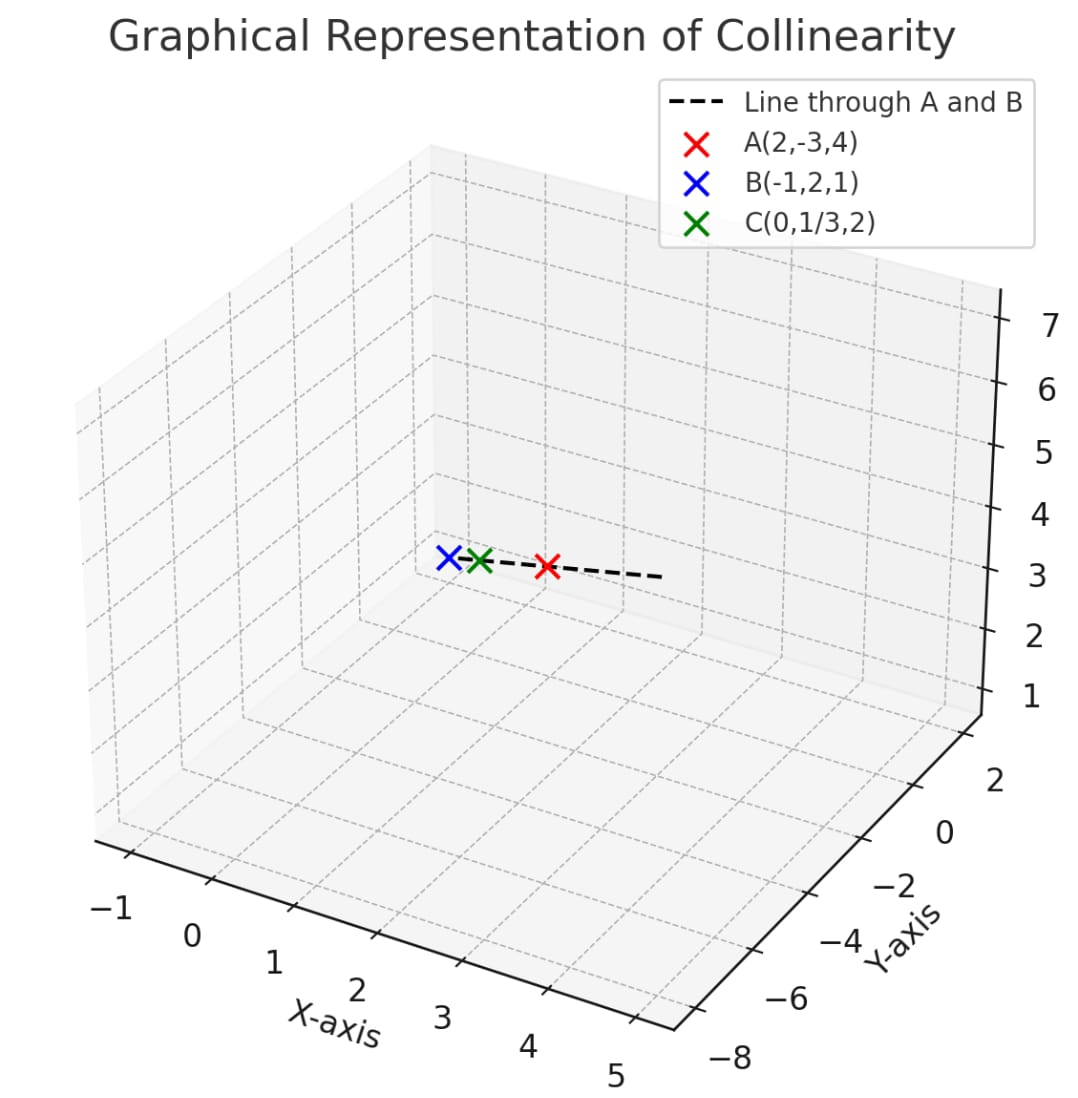
\includegraphics[width=0.6\linewidth]{figs/image.png}
    \caption{Image Visual}
    \label{fig:figs/image.png}
\end{figure}

\end{document}

